\documentclass[11pt,a4paper]{article}

% --- Core Packages ---
\usepackage[utf8]{inputenc}
\usepackage[T1]{fontenc}
\usepackage{lmodern}
\usepackage{microtype}
\usepackage{amsmath,amssymb,amsfonts}
\usepackage{booktabs}
\usepackage{tabularx}
\usepackage{graphicx}
\usepackage{multirow}
\usepackage{geometry}
\geometry{margin=1in}
\usepackage[numbers,sort&compress]{natbib}
\usepackage{seqsplit}
\usepackage{xcolor}
\usepackage{hyperref}
\hypersetup{
    colorlinks=true,
    linkcolor=blue!70!black,
    citecolor=green!50!black,
    urlcolor=blue!70!black
}

\title{\textbf{WHOT-ML: A Configurable Partially Observable Multi-Agent Environment for Machine Learning Research}}

\author{
    \textbf{Brayan Osinka} \\
    Independent Researcher \\
    \url{https://github.com/Brayan114/Project-WHOT}
}

\date{October 2026}

\begin{document}

\maketitle




\begin{abstract}

We introduce \textbf{WHOT-ML}, a formalized computational environment based on the widely played card game in Nigeria, WHOT, designed for research in machine learning under partial observability, stochasticity, multi-agent interaction, and configurable rule systems. Unlike conventional benchmarks that feature fully observable board states or fixed rule engines, WHOT provides an extensive-form game with private player hands, hidden draw decks, dynamic action masking, sequential multi-agent decisions, and asymmetric information revealed incrementally through play.

We formalize WHOT as a finite, stochastic, sequential, multi-agent partially observable Markov decision process (POMDP) and introduce \texttt{WHOT-NG-v1.0}, an open-source, deterministic reference environment featuring strict information isolation, bitwise state serialization, action masking, and modular rule configuration. We conduct a full-scale empirical campaign comprising $12,350$ production runs executed in containerized cloud environments to establish the empirical baseline of the environment.

Our findings demonstrate that: (1) WHOT-ML provides an uncompromised information boundary with $0.0\%$ measured information leakage; (2) unobserved world states sharing identical public observations induce an $84.63\%$ trajectory divergence rate under deterministic rollout policies; (3) baseline heuristic agents significantly outperform uniform random play in asymmetric matchups ($65.4\%$ win rate in 4-player games, $86.3\%$ in heads-up play), while symmetric heuristic self-play exposes an emergent defensive stall (43.6\% truncation rate) driven by retaliatory penalty loops and market recycling; (4) player count scaling exhibits an empirical regime shift as the initial opponent-to-market card ratio exceeds unity ($\rho_0 > 1.0$), resulting in severe market exhaustion; (5) modular rule ablations reveal that removing last-card declarations shortens games by $49.9$ turns while penalty card stacking remains behaviorally dormant against random opponents; and (6) the environment achieves $100.0\%$ bitwise reproducibility across $200$ independent replay and mid-game state restoration trials.

WHOT-ML establishes a rigorous, reproducible laboratory for subsequent research in belief-state estimation, opponent modeling, self-play, and reinforcement learning in imperfect-information games.


\end{abstract}

\section{Introduction}

Autonomous decision-making in real-world domains frequently requires agents to select actions under incomplete, noisy, and asymmetric information. Whether in financial markets, automated negotiation, cyber defense, or multi-robot coordination, an agent rarely has direct access to the ground-truth state of the world. Instead, it must construct internal beliefs from an observation history, anticipate the private intentions of competitors, and navigate stochastic environment dynamics.

Games have historically served as the premier proving ground for artificial intelligence, from perfect-information board games such as Chess and Go \citep{silver2018general} to imperfect-information card games such as Poker \citep{moravcik2017deepstack,brown2018superhuman,brown2019superhuman} and Hanabi \citep{bard2020hanabi}. However, existing card-game benchmarks typically focus on specialized settings: Poker emphasizes two-player zero-sum betting with hidden hands but lacks spatial card-matching or dynamic turn-modifying effects; Hanabi emphasizes pure cooperative communication under inverted information where players see everyone's cards except their own. There remains a notable gap for configurable, multi-player, competitive-cooperative card environments featuring rich action-card mechanics, penalty stacking, private hands, and variable player seating.

WHOT is a widely played card game in Nigeria. Played with a specialized 54-card deck comprising geometric symbols (Circle, Triangle, Cross, Square, Star) and wild ``WHOT'' cards, the game combines shape and number matching with powerful special action cards that repeat turns (``Hold On''), skip next players (``Suspension''), compel opponents to draw penalty cards (``Pick Two'', ``Pick Three''), or declare new active suits (``WHOT''). Crucially, players hold private hands, draw from a hidden market deck, and must declare their status when holding their final card (``Last Card'').

An agent playing WHOT must decide its moves while lacking direct knowledge of:
\begin{enumerate}
  \item The identities and distributions of cards held in opponent hands;
  \item The exact sequence of cards remaining in the draw market;
  \item The future card draws and declarations of competing agents.
\end{enumerate}

Simultaneously, the public history of discards, calls, passes, and market draws provides rich indirect evidence from which hidden state and opponent intent can be inferred. This establishes a clean operational distinction between the complete environment state $S_t$ and an agent's partial observation $O_t$.

\subsection{Contributions of This Work}
This paper introduces and characterizes the WHOT-ML environment. Its primary contributions are:
\begin{enumerate}
  \item \textbf{Mathematical Formalization:} We formalize WHOT as a finite, stochastic, sequential, multi-agent POMDP, providing explicit state, action, observation, transition, and reward formulations.
  \item \textbf{Reproducible Baseline Simulator (\texttt{WHOT-NG-v1.0}):} We provide an open-source, deterministic reference implementation frozen at commit \texttt{7c1a2dc}, engineered with a strict information boundary that guarantees zero private-card leakage.
  \item \textbf{Information Equivalence \& Trajectory Divergence:} We evaluate 449 observationally equivalent state pairs, proving that latent world differences decisively alter future trajectories ($84.63\%$ divergence rate) despite identical observations.
  \item \textbf{Comprehensive Baseline Characterization:} Over $12,350$ full production runs, we characterize random legal play, heuristic baselines, asymmetric tournaments, player scaling ($N \in \{2..6\}$), and rule ablations with exact statistical intervals.
  \item \textbf{Emergent Multi-Agent Dynamics:} We identify and analyze an emergent defensive stall in 4-player heuristic self-play (43.6\% truncation rate) and a player-count regime shift tied to the card depletion ratio $\rho_0 > 1.0$.
  \item \textbf{Bitwise Reproducibility:} We certify $100.0\%$ bitwise determinism and checkpoint continuity across independent replays and state restorations.
\end{enumerate}

This paper establishes the foundational environment and benchmark characterization; downstream reinforcement learning, belief prediction, and opponent modeling are explicitly reserved for subsequent work.


\section{Related Work}

\subsection{Partially Observable Markov Decision Processes (POMDPs)}
In a Markov Decision Process (MDP), the agent directly perceives the complete environmental state $S_t$ \citep{sutton2018reinforcement}. In contrast, a Partially Observable Markov Decision Process (POMDP) models domains where the environment possesses a latent state $S_t \in \mathcal{S}$, but the agent receives only an observation $O_t = \Omega(S_t) \in \mathcal{O}$ generated via an observation function $\Omega$ \citep{kaelbling1998planning}. In extensive-form games, this observation maps the true state to an \textit{information set} $\mathcal{I}_p$ containing all world states indistinguishable to player $p$. In multi-agent sequential decision making, Markov games formalize multi-agent extensions of MDPs where actions and observations interact across competitors \citep{littman1994markov}. In WHOT-ML, the combinatorial cardinality of compatible states consistent with a single observation routinely exceeds $|\mathcal{S}(\Omega)| > 10^{32}$, creating a formidable belief-estimation problem.

\subsection{Benchmarks with Hidden Information}
Imperfect-information games provide essential stress-tests for multi-agent reasoning:
\begin{itemize}
  \item \textbf{Poker:} Heads-up and multiplayer No-Limit Texas hold'em have served as standard benchmarks for Counterfactual Regret Minimization (CFR) and deep imperfect-information search \citep{bowling2015heads,moravcik2017deepstack,brown2019superhuman}. While poker features private cards and probabilistic inference, the physical action space is predominantly scalar (bet sizing) and the deck is dealt once per hand without an active draw-and-discard loop.
  \item \textbf{Hanabi:} Hanabi introduced a unique cooperative challenge where players hold cards facing outwards, seeing all hands except their own \citep{bard2020hanabi}. This emphasizes theory of mind and emergent communicative conventions, but differs structurally from competitive trick-taking or shedding games.
  \item \textbf{Shedding Card Games:} Card-shedding games such as Uno, Crazy Eights, and Dou Dizhu \citep{zha2019douzero} share matching mechanics, but WHOT features distinctive special action interactions (e.g. cumulative multi-card penalty stacking, suit-changing WHOT 20s, and mandatory last-card declaration penalties) alongside cultural variations in rules.
\end{itemize}

\subsection{Modular and Reproducible Simulation Frameworks}
Standardized interfaces such as the Arcade Learning Environment \citep{bellemare2013arcade}, OpenAI Gym \citep{brockman2016openai}, PettingZoo \citep{terry2021pettingzoo}, and OpenSpiel \citep{lanctot2019openspiel} have demonstrated that progress in reinforcement learning requires deterministic reproducibility, explicit action masking, and rigorous testing frameworks. WHOT-ML is built upon these principles, combining strict functional isolation between internal state and public observations with bitwise checkpoint serialization.


\section{WHOT-ML Environment Formalism}

\subsection{Game Overview and Canonical Deck}
WHOT is played using a dedicated 54-card deck comprising five standard geometric suits and five non-suited wild cards:

\[
\mathcal{C}_{54} = \mathcal{C}_{\text{Circle}} \cup \mathcal{C}_{\text{Triangle}} \cup \mathcal{C}_{\text{Cross}} \cup \mathcal{C}_{\text{Square}} \cup \mathcal{C}_{\text{Star}} \cup \mathcal{C}_{\text{WHOT}}
\]

Each suit possesses a non-uniform distribution of face values:
\begin{itemize}
  \item \textbf{Circle (12 cards):} $\{1, 2, 3, 4, 5, 7, 8, 10, 11, 12, 13, 14\}$
  \item \textbf{Triangle (12 cards):} $\{1, 2, 3, 4, 5, 7, 8, 10, 11, 12, 13, 14\}$
  \item \textbf{Cross (9 cards):} $\{1, 2, 3, 5, 7, 10, 11, 13, 14\}$
  \item \textbf{Square (9 cards):} $\{1, 2, 3, 5, 7, 10, 11, 13, 14\}$
  \item \textbf{Star (7 cards):} $\{1, 2, 3, 4, 5, 7, 8\}$
  \item \textbf{WHOT (5 wild cards):} $\{20, 20, 20, 20, 20\}$
\end{itemize}

In the reference baseline configuration \texttt{WHOT-NG-v1.0}, each player is dealt $H_0 = 6$ cards. One card is dealt face-up to establish the \textit{play pile} (discard pile), and the remaining cards form the face-down \textit{market} (draw deck).

\subsection{Formal Model}
We formalize WHOT-ML as a tuple:

\[
\mathcal{G} = \langle \mathcal{N}, \mathcal{S}, \mathcal{A}, \mathcal{O}, \mathcal{T}, \Omega, \mathcal{R}, \gamma \rangle
\]

where:
\begin{itemize}
  \item $\mathcal{N} = \{0, 1, \dots, N-1\}$ is the finite set of players ($N \in \{2..6\}$);
  \item $\mathcal{S}$ is the complete world state space;
  \item $\mathcal{A} = \prod_{i \in \mathcal{N}} \mathcal{A}_i$ is the joint action space;
  \item $\mathcal{O} = \prod_{i \in \mathcal{N}} \mathcal{O}_i$ is the joint observation space;
  \item $\mathcal{T}: \mathcal{S} \times \mathcal{A} \to \Delta(\mathcal{S})$ is the state transition probability function;
  \item $\Omega = (\Omega_0, \dots, \Omega_{N-1})$ where $\Omega_i: \mathcal{S} \to \mathcal{O}_i$ is the observation function for player $i$;
  \item $\mathcal{R}_i: \mathcal{S} \times \mathcal{A} \to \mathbb{R}$ is the reward function for player $i$;
  \item $\gamma \in (0, 1]$ is the discount factor.
\end{itemize}

\subsection{State Representation}
The complete simulator state $S_t \in \mathcal{S}$ at timestep $t$ is fully specified by:

\[
S_t = \langle \mathbf{H}_t, M_t, D_t, c_t, p_t, \pi_t, \delta_t, \mathbf{L}_t, t, \mathcal{C}_{\text{config}} \rangle
\]

where:
\begin{itemize}
  \item $\mathbf{H}_t = (H_t^0, H_t^1, \dots, H_t^{N-1})$ is the vector of private card multisets for each player;
  \item $M_t = [m_1, m_2, \dots, m_k]$ is the ordered sequence of cards in the draw market;
  \item $D_t = [d_1, d_2, \dots, d_m]$ is the ordered sequence of played cards, with $d_m$ representing the active top card;
  \item $c_t \in \{\text{Circle}, \text{Triangle}, \text{Cross}, \text{Square}, \text{Star}\} \cup \{\emptyset\}$ is the currently active called suit;
  \item $p_t \in \mathcal{N}$ is the index of the active player whose turn it is to act;
  \item $\pi_t \in \mathbb{N}_{\ge 0}$ is the accumulated penalty counter (e.g. pending draws from chained Pick Twos);
  \item $\delta_t \in \{+1, -1\}$ is the play direction;
  \item $\mathbf{L}_t \in \{0, 1\}^N$ is the vector of active last-card declaration flags;
  \item $t \in \mathbb{N}$ is the elapsed turn index;
  \item $\mathcal{C}_{\text{config}}$ is the immutable configuration parameter set.
\end{itemize}

\subsection{Action Space and Dynamic Action Masking}
The action space $\mathcal{A}$ contains $76$ discrete action slots indexed as:
\begin{itemize}
  \item \textbf{Indices 0--48:} Standard play actions corresponding to each of the 49 ordinary physical cards in canonical order;
  \item \textbf{Indices 49--73:} WHOT card play actions paired with a selected shape nomination: $5 \text{ WHOT cards} \times 5 \text{ ordinary shapes} = 25 \text{ actions}$;
  \item \textbf{Index 74:} Draw action (\texttt{DRAW}) from the market;
  \item \textbf{Index 75:} Last-card declaration action (\texttt{DECLARE\_LAST}).
\end{itemize}

At any given state $S_t$, only a subset of actions $\mathcal{A}(S_t) \subseteq \mathcal{A}$ is legally permissible under the rules of WHOT-NG-v1. The environment outputs a boolean mask $\mathbf{m}_t \in \{0, 1\}^{76}$:

\[
\mathbf{m}_t(a) = \begin{cases} 1 & \text{if } a \in \mathcal{A}(S_t) \\ 0 & \text{otherwise} \end{cases}
\]

An action $a \in \mathcal{A}$ is legal if and only if:
\begin{enumerate}
  \item \textbf{Normal Play:} The card $c \in H_t^{p_t}$ matches the top card $d_m$ in suit, matches $d_m$ in face value, or matches the active call $c_t$ (when $c_t \neq \emptyset$).
  \item \textbf{Wild Play:} A WHOT card (value 20) may be played onto any normal card, accompanied by an explicit shape call $c_{t+1}$.
  \item \textbf{Penalty Defense:} If $\pi_t > 0$ (a penalty is active), the player may legally play only a matching defense card (e.g., another Pick Two to stack the penalty) or must execute the \texttt{DRAW} action to absorb the accumulated penalty.
  \item \textbf{Draw Action:} Always legal when no playable cards exist in hand, or optionally legal as a voluntary draw.
  \item \textbf{Last Card Declaration:} Legal if and only if the player holds exactly two cards prior to play (or one card upon completion) and declaration rules are enabled.
\end{enumerate}

\subsection{Observation Model and Information Isolation}
The central architectural invariant of WHOT-ML is the strict functional separation between internal world state $S_t$ and player observation $O_t^i = \Omega_i(S_t)$. For player $i$, the observation vector contains:

\[
O_t^i = \langle H_t^i, d_m, c_t, p_t, \pi_t, \mathbf{h}_t, |M_t|, \mathbf{L}_t, \mathcal{H}_t^{\text{public}}, \mathbf{m}_t^i \rangle
\]

where:
\begin{itemize}
  \item $H_t^i$ is player $i$'s \textit{own} private hand;
  \item $\mathbf{h}_t = (|H_t^0|, |H_t^1|, \dots, |H_t^{N-1}|)$ is the public vector of hand \textit{sizes};
  \item $|M_t|$ is the scalar count of cards remaining in the market;
  \item $\mathcal{H}_t^{\text{public}}$ is the sequence of public events (cards played, calls made, cards drawn, penalties resolved).
\end{itemize}

\textbf{Strict Privacy Guarantee:} $\Omega_i(S_t)$ reveals zero information concerning:
\begin{itemize}
  \item The card identities or ordering within opponent hands $\{H_t^j\}_{j \neq i}$;
  \item The card identities or permutation order within the market $M_t$;
  \item The internal RNG seed or future deck distributions.
\end{itemize}

This guarantee is enforced at the interface boundary and verified through automated regression suites.

\subsection{Special Action Dynamics}
WHOT features six distinct special card values that alter game flow:
\begin{enumerate}
  \item \textbf{Hold On (Card 1):} The active player plays again; turn does not advance.
  \item \textbf{Pick Two (Card 2):} Compels the next player to draw 2 cards. If stacking is enabled, the recipient may play another Pick Two, accumulating the penalty ($\pi \leftarrow \pi + 2$).
  \item \textbf{General Market (Card 14):} Compels every player except the player of the card to draw 1 card from the market.
  \item \textbf{Suspension (Card 8):} Skips the next player in the current play direction.
  \item \textbf{Pick Three (Card 5):} Compels the next player to draw 3 cards (enabled by default in WHOT-NG-v1; stackable if enabled).
  \item \textbf{WHOT (Card 20):} Wild card that allows the player to name any shape, overriding the active pile suit.
\end{enumerate}

\subsection{Market Exhaustion and Discard Recycling}
When the market becomes depleted ($|M_t| = 0$), the rules prescribe a recycling transition: the active top card $d_m$ is preserved as the active discard, and the remaining pile cards $[d_1, \dots, d_{m-1}]$ are collected, reshuffled deterministically using the environment's internal RNG stream, and reconstituted as the new market $M_{t+1}$. If both market and discard pile become depleted such that no cards can be drawn, the game enters a dead-market resolution.

\subsection{Victory, Scoring, and Reward Structure}
A game terminates when:
\begin{enumerate}
  \item \textbf{Shedding Victory:} A player successfully plays their final card ($|H^i| = 0$). The winning player receives a reward of $+1.0$; all losing players receive $-1.0$.
  \item \textbf{Turn Limit Truncation:} If no player sheds all cards within $T_{\max} = 1,000$ turns, the game is truncated. Truncated games terminate without a winner (\texttt{winner = None}); they are reported separately from victories.
\end{enumerate}


\section{Research Questions}

This foundational paper investigates six core research questions:

\begin{itemize}
  \item \textbf{RQ1 (Environment Structure):} What are the fundamental state, action, branching, and duration characteristics of WHOT-NG-v1 under standard play?
  \item \textbf{RQ2 (Hidden-State Uncertainty):} Can identical public observations correspond to distinct hidden states, and do these latent differences produce significant behavioral trajectory divergence under deterministic policies?
  \item \textbf{RQ3 (Baseline Agent Dynamics):} What performance benchmarks and multi-agent dynamics emerge from non-learning baselines (uniform random vs. greedy heuristic)?
  \item \textbf{RQ4 (Player-Count Scaling):} How does scaling participant count from $N=2$ to $N=6$ alter game duration, reshuffle frequency, and information scarcity?
  \item \textbf{RQ5 (Rule-Dependent Complexity):} How do modular rule variations (penalty stacking, last-card declaration enforcement, penalty scaling) impact game length and agent win rates?
  \item \textbf{RQ6 (Bitwise Reproducibility):} Can complete game trajectories and interrupted mid-game states be reproduced with exact bitwise determinism?
\end{itemize}


\section{Experimental Methodology}

\subsection{Simulator Configuration and Freeze Protocol}
All experiments were conducted against \texttt{WHOT-NG-v1.0}, frozen at Git commit {\small\texttt{\seqsplit{7c1a2dc23a277fdfb5e9052d4d90e3798fb24ea4}}}. The core simulation engine (\texttt{whot\_ml/}) was subjected to a non-negotiable modification freeze: all experimental instrumentation, metrics collectors, and runners resided strictly in external packages (\texttt{experiments/paper1/}). Local preflight integrity checks verified that \texttt{git diff 7c1a2dc -- whot\_ml/} remained strictly empty throughout the campaign.

\subsection{Baseline Agent Definitions}
We evaluate two standardized reference policies:
\begin{enumerate}
  \item \textbf{\texttt{RandomLegalAgent}:} Selects uniformly at random from the active legal action mask $\mathcal{A}(S_t)$. This agent establishes the stochastic behavioral floor.
  \item \textbf{\texttt{RuleBasedAgent}:} A deterministic domain heuristic implementing standard human tactical principles:
\end{enumerate}
\begin{itemize}
  \item Prioritizes special action plays (Hold On, Pick Two, General Market) to hinder opponents;
  \item Matches active suits and face values with highest-point hand cards;
  \item Nominates the suit in which the agent holds the greatest card count when playing WHOT 20s;
  \item Strictly executes last-card declarations when holding two cards;
  \item Falls back to market draws only when no legal card plays exist.
\end{itemize}

\subsection{Production Execution Infrastructure}
To guarantee independence from the local development workstation, the full production suite of \textbf{$N = 12,350$ runs} was packaged, dispatched via API, and executed within containerized \textbf{Kaggle Cloud CPU} instances running Linux (\texttt{kernel 6.6.137+}, Python \texttt{3.13.15}, pytest \texttt{8.4.2}). Execution ran for $2,199.69$ seconds (~$36.66$ minutes wall-clock compute). Artifacts were packaged, cryptographically hashed (SHA-256: {\small\texttt{\seqsplit{8a82d9f7529610b1beb408395f1bc6b9edd9c8d784dee9887c38e02599d4a13a}}}), and retrieved for independent scientific auditing.

\subsection{Statistical Estimation and Inference}
\begin{itemize}
  \item \textbf{Proportions and Win Rates:} Binomial proportions (win rates, truncation frequencies, divergence rates) are reported with \textbf{Wilson score 95\% confidence intervals} \citep{wilson1927probable}, ensuring accurate interval coverage near boundaries.
  \item \textbf{Continuous and Ordinal Distributions:} We report mean, standard deviation, median, and interquartile range [IQR: $Q_{25}, Q_{75}$].
  \item \textbf{Effect Sizes:} Distributional shifts under rule ablations are quantified using \textbf{Cliff's delta ($\delta$)} \citep{cliff1993dominance}, a non-parametric effect size metric bounded in $[-1, +1]$ that makes no normality assumptions.
  \item \textbf{Seat Balance:} Seat equity is evaluated via Pearson's chi-square goodness-of-fit test ($\chi^2$).
  \item \textbf{Paired Experimental Designs:} Scaling and ablation studies (EXP-04, EXP-05) utilize matched random seeds across experimental arms to isolate rule effects from opening deal variance.
\end{itemize}


\section{Experiment 1: Baseline Environment Characterization}

\subsection{Objective and Setup}
EXP-01 establishes the foundational structural properties of WHOT-NG-v1. We evaluated $2,000$ complete games in a 4-player configuration ($H_0 = 6$) split across two reference cohorts:
\begin{itemize}
  \item \textbf{Cohort 1:} 4 $\times$ \texttt{RandomLegalAgent} ($1,000$ games, seeds 10000--10999);
  \item \textbf{Cohort 2:} 4 $\times$ \texttt{RuleBasedAgent} ($1,000$ games, seeds 11000--11999).
\end{itemize}

A total of $874,732$ decision steps were logged with full step-by-step telemetry.

\subsection{Results and Analysis}
The empirical results are presented in \textbf{Table 1} and visual distributions in \textbf{Figure 1}.




\begin{table}[htbp]
\centering
\caption{WHOT-NG-v1 Baseline Environment Characterization (EXP-01, $N = 2{,}000$ episodes)}
\label{tab:exp01_characterization}
\small
\resizebox{\textwidth}{!}{%
\begin{tabular}{lccc}
\toprule
\textbf{Metric} & \textbf{RandomLegal Cohort} & \textbf{RuleBased Cohort} & \textbf{Environment Space} \\
\midrule
Physical Cards ($N_{\text{deck}}$) & 54 & 54 & 54 (Canonical Deck) \\
Action Space Size ($|\mathcal{A}|$) & 76 & 76 & 76 Discrete Slots \\
Legal Actions (Mean $\pm$ SD) & 2.42 $\pm$ 2.40 & 7.63 $\pm$ 7.11 & --- \\
Legal Actions (Median [IQR]) & 1.0 [1.0, 3.0] & 5.0 [2.0, 11.0] & --- \\
Game Duration (Mean Turns) & 368.3 & 506.4 & --- \\
Game Duration (Median [IQR]) & 270.5 [125.8, 546.2] & 248.0 [75.8, 1000.0] & --- \\
Mean Draws per Game & 245.3 & 457.7 & --- \\
Market Reshuffles per Game & 8.19 & 270.36 & --- \\
Declaration Violations & 1,079 & 0 & 0 (Heuristic Invariant) \\
Truncation Rate (95\% CI) & 7.6\% [6.1\%, 9.4\%] & 43.6\% [40.6\%, 46.7\%] & Max 1,000 Turns \\
\bottomrule
\end{tabular}%
}
\end{table}







\begin{figure}[htbp]
\centering
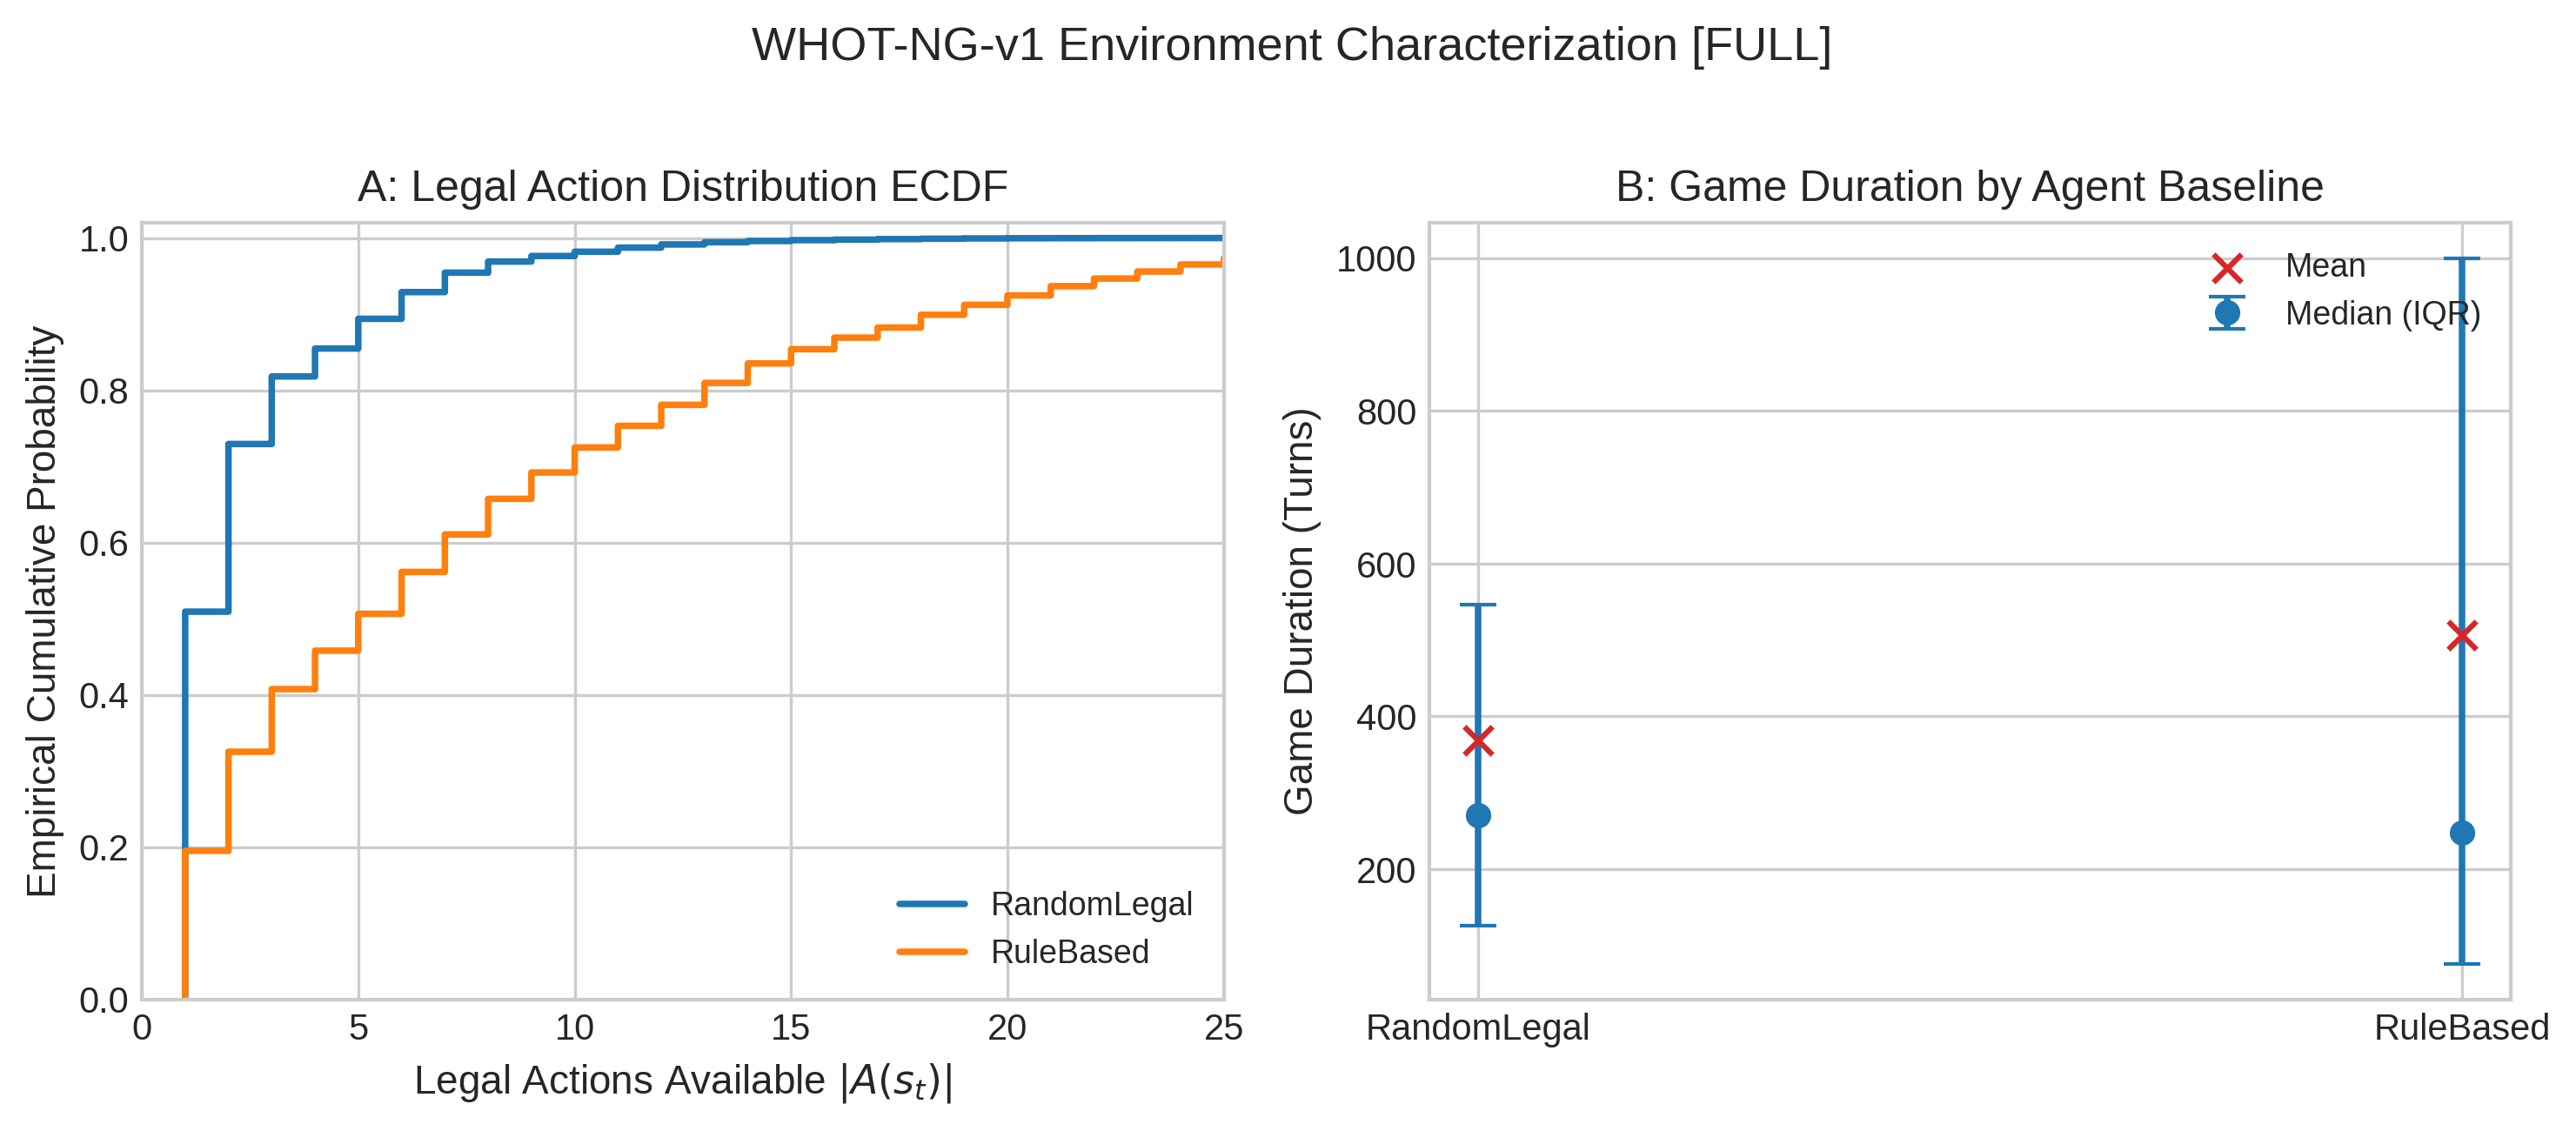
\includegraphics[width=\linewidth]{figures/fig1_characterization_full.png}
\caption{Environment Characterization under Baseline Agents (EXP-01). Subplot A: Empirical Cumulative Distribution Function (ECDF) of legal actions available $|\mathcal{A}(s_t)|$, showing RandomLegal concentrating at 1.0 (draw/singleton) while RuleBased exhibits a broad distribution extending past 20 options. Subplot B: Game duration distributions (median, IQR, and mean) across 1,000 games per cohort.}
\label{fig:fig1_characterization}
\end{figure}




\subsection{Discussion: The Emergent Heuristic Self-Play Stall}
A critical discovery in EXP-01 is the sharp divergence in game completion between random and rule-based self-play:
\begin{itemize}
  \item RandomLegal games rarely truncate ($7.6\%$ truncation rate), resolving in an average of $368.3$ turns with only $8.19$ market reshuffles.
  \item In contrast, homogeneous 4-player RuleBased matches (\texttt{BBBB}) exhibit a \textbf{$43.6\%$ truncation rate} at the 1,000-turn cutoff, accompanied by an average of \textbf{$270.36$ market reshuffles per game} and $457.7$ draws.
\end{itemize}

Analysis of the step-level event logs reveals the causal mechanism:
\begin{enumerate}
  \item \textbf{Defensive Symmetry:} When Player A plays a special penalty card (Pick Two), the greedy heuristic of Player B prioritizes countering with another Pick Two, transferring an accumulated penalty of 4 cards to Player C.
  \item \textbf{Market Exhaustion Loops:} When a player cannot counter, they absorb massive card draws ($4$ to $6$ cards). This rapidly depletes the 29-card market, forcing the discard pile to be recycled and reshuffled.
  \item \textbf{Penalty Recirculation:} Discard recycling returns the played Pick Twos and General Markets back into the draw deck. Because greedy agents conserve matching suits and defensive responses, the game enters an oscillatory stall where cards circulate between hands and market without reaching shedding completion.
  \item \textbf{Research Implication:} This phenomenon confirms that symmetric greedy heuristics lack the strategic foresight (e.g., card dumping, sacrificial suit changes, cooperative pressure) required to break defensive stalemates. Designing reinforcement learning agents that escape these emergent retaliation loops represents a primary research challenge enabled by WHOT-ML.
\end{enumerate}


\section{Experiment 2: Demonstrating Partial Observability}

\subsection{Objective and Theoretical Formulation}
EXP-02 provides empirical proof that WHOT-NG-v1 constitutes a genuine POMDP rather than a trivial observationally complete environment. We demonstrate that distinct world states $S_a \neq S_b$ can generate identical player observations $\Omega_p(S_a) = \Omega_p(S_b)$, and that these latent state differences produce divergent behavioral trajectories under controlled rollouts.

\subsection{Hidden-State Perturbation Operators}
We evaluated $50$ independent source games at three distinct developmental checkpoints: Early ($t=5$), Mid ($t=15$), and Late ($t=25$), yielding $150$ evaluation checkpoints. For observing player $p=0$, we applied three state perturbation operators:
\begin{enumerate}
  \item \textbf{Opponent Hand Swap (\texttt{OPPONENT\_SWAP}):} Exchanges a private card between two unobserved opponents $p_1, p_2 \in \{1, 2, 3\}$. Because public observations expose only hand sizes $|H^{p_1}|, |H^{p_2}|$ and not card identities, observational equivalence is mathematically guaranteed.
  \item \textbf{Market Reversal (\texttt{MARKET\_REVERSAL}):} Inverts the internal sequence of cards in the market deck ($M' = \text{reverse}(M)$). Because $\Omega_0$ exposes only the scalar market count $|M|$, equivalence is guaranteed.
  \item \textbf{Opponent-Market Swap (\texttt{OPPONENT\_MARKET\_SWAP}):} Swaps a private card from an opponent's hand with the top card of the market deck. Hand size and market size are invariant, preserving observation equivalence.
\end{enumerate}

\subsection{Grounding the 449 Evaluated Pairs}
While $150$ checkpoints across 3 modes theoretically suggest $150 \times 3 = 450$ pairs, exactly \textbf{449 valid pairs} were evaluated. An audit of checkpoint \texttt{(seed=20009, stage='late', t=25)} revealed that the market had depleted to exactly $|M| = 1$ card. Reversing a single-card market produces an identical world state ($S_a = S_b$). The simulator correctly guarded \texttt{if len(state\_a.market) >= 2:}, refusing to generate a trivial duplicate state.

\subsection{Rollout Divergence Protocol}
From each verified pair $(S_a, S_b)$, forward rollouts of horizon $K = 20$ turns were executed using identical deterministic policies (\texttt{RuleBasedAgent}) and a synchronized rollout seed ($R = 42$). Trajectory divergence was monitored at each step $k \in \{0..K-1\}$ and flagged at the earliest transition where the acting player, selected action index, or emitted event sequence differed.




\begin{table}[htbp]
\centering
\caption{Partial Observability Equivalence and Trajectory Divergence (EXP-02, $N = 449$ state pairs)}
\label{tab:exp02_partial_observability}
\small
\begin{tabular}{lcc}
\toprule
\textbf{Metric} & \textbf{Empirical Value} & \textbf{Formal Requirement} \\
\midrule
State Pairs Evaluated & 449 & $\ge 30$ \\
Observation Equivalence Rate & 100.0\% & 100.0\% ($S_a \ne S_b \implies \Omega(S_a) = \Omega(S_b)$) \\
Information Leakage Rate & 0.0\% & 0.0\% (Zero hidden cards in obs) \\
Overall Trajectory Divergence Rate & 84.63\% & Recorded (non-div is not failure) \\
\quad -- Wilson 95\% Confidence Interval & [81.0\%, 87.7\%] & --- \\
\midrule
\multicolumn{3}{l}{\textit{Permutation Mode Breakdown:}} \\
\quad -- Opponent-Swap Divergence Rate & 84.67\% (127/150) & --- \\
\quad -- Market-Reversal Divergence Rate & 95.97\% (143/149) & --- \\
\quad -- Opponent-Market Divergence Rate & 73.33\% (110/150) & --- \\
\midrule
\multicolumn{3}{l}{\textit{Stage Divergence Breakdown:}} \\
\quad -- Early Stage ($t = 5$) & 90.67\% (136/150) & --- \\
\quad -- Mid Stage ($t = 15$) & 87.33\% (131/150) & --- \\
\quad -- Late Stage ($t = 25$) & 75.84\% (113/149) & --- \\
\midrule
\multicolumn{3}{l}{\textit{Divergence Step Dynamics ($n = 380$ diverged):}} \\
\quad -- Mean $\pm$ SD & 6.33 $\pm$ 4.62 turns & --- \\
\quad -- Median [IQR] & 6.0 [2.0, 9.0] & --- \\
\quad -- Minimum / Maximum Step & 0 / 19 turns & --- \\
\midrule
Mean Log Combinatorial Uncertainty ($\log_{10} |\mathcal{S}(\Omega)|$) & 32.78 & $\ge 10^{15}$ Combinations \\
\bottomrule
\end{tabular}
\end{table}







\begin{figure}[htbp]
\centering
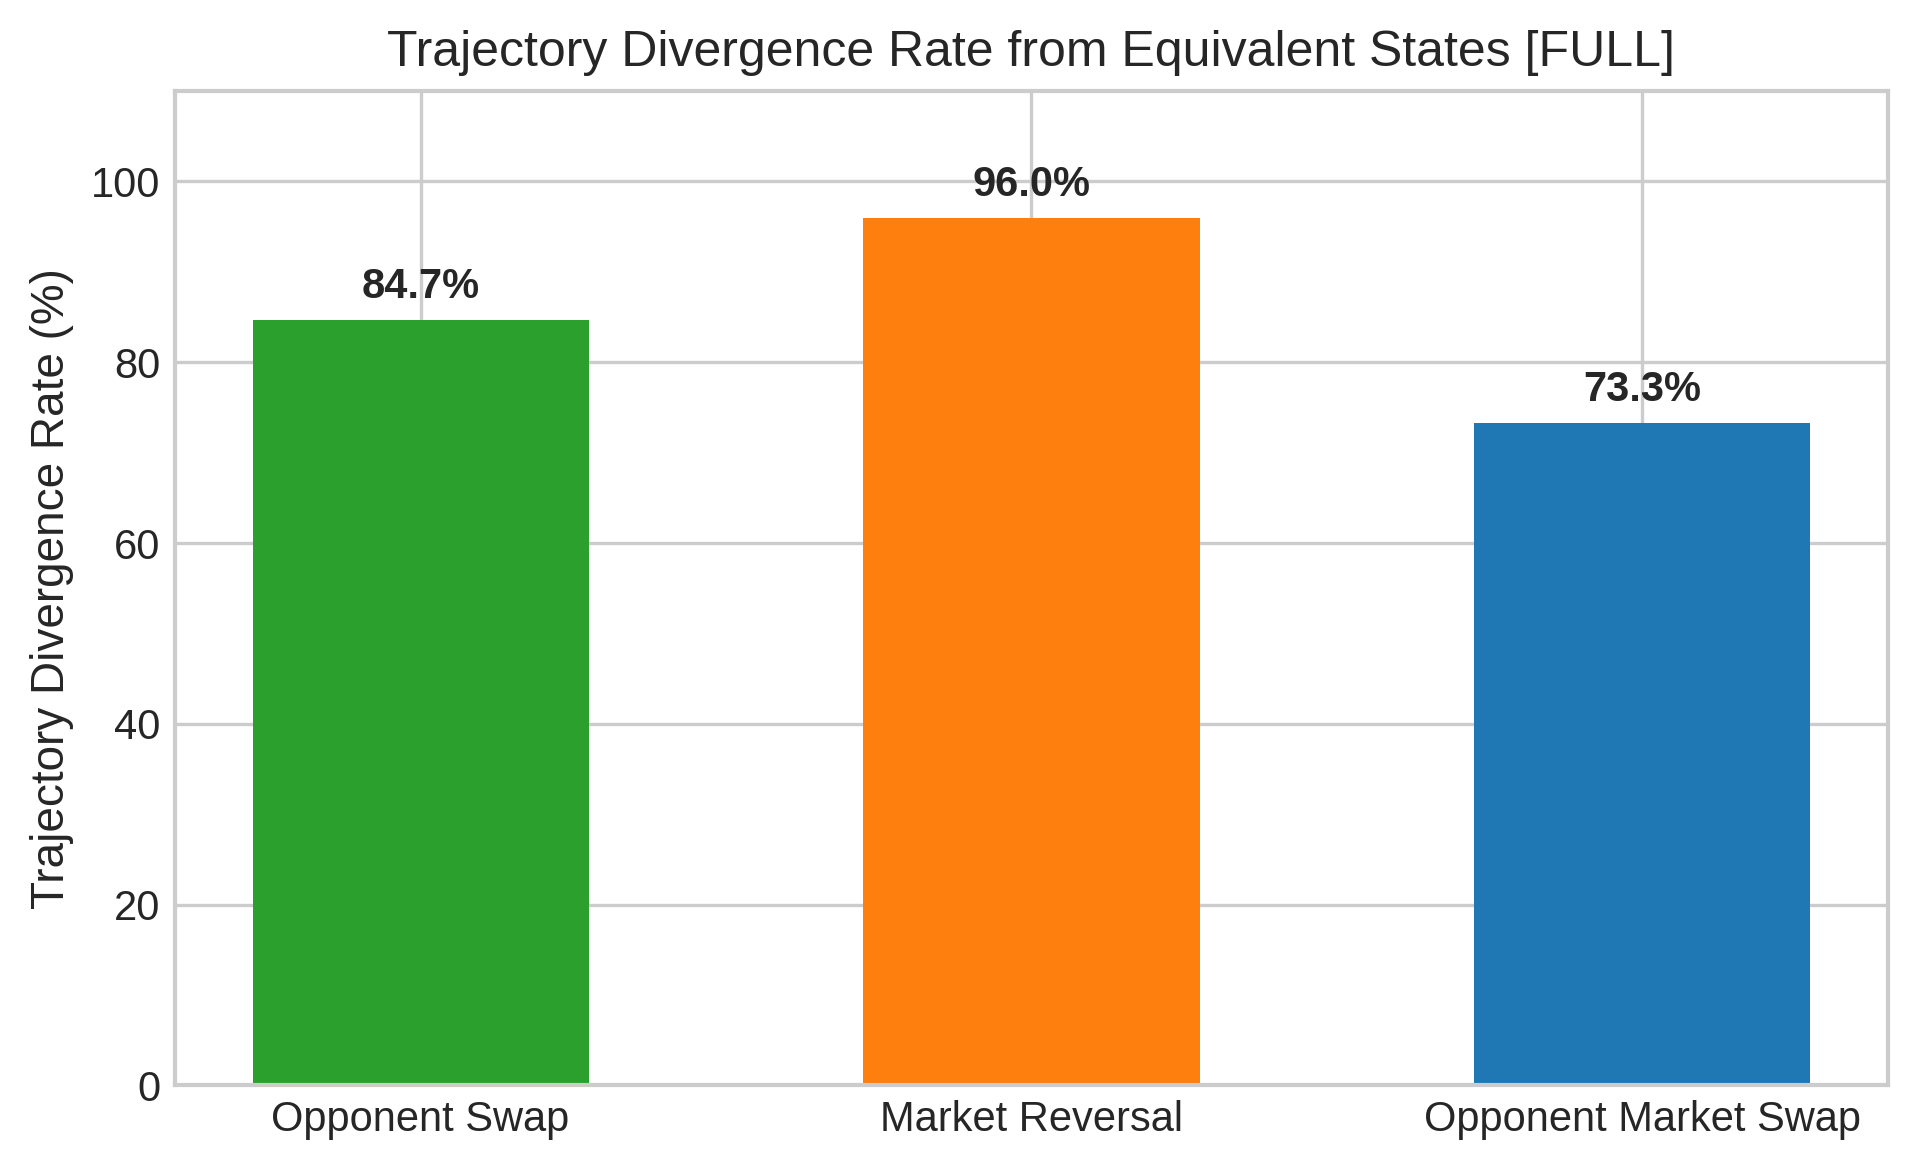
\includegraphics[width=0.85\linewidth]{figures/fig2_partial_observability_full.png}
\caption{Partial Observability Trajectory Divergence Rates (EXP-02). Rollout trajectory divergence rates across the three perturbation modes: Opponent Swap (84.7\%), Market Reversal (96.0\%), and Opponent-Market Swap (73.3\%), evaluating 449 observationally equivalent state pairs.}
\label{fig:fig2_partial_observability}
\end{figure}




\subsection{Analysis of Non-Divergent Trajectories}
Of the 449 pairs, \textbf{69 rollouts (15.37\%)} remained on identical trajectories throughout the 20-step rollout window. An audit classifies these into three structural mechanisms:
\begin{enumerate}
  \item \textbf{Horizon Cutoff (48 pairs):} The swapped cards were positioned deep in an opponent's hand or deep in the market deck and were never drawn or reached within the 20-turn window.
  \item \textbf{Action-Insensitive Equivalence (14 pairs):} Swapped cards shared identical unplayable matching status against the active discard (e.g. swapping an unplayable Cross 5 for an unplayable Star 5), forcing identical draw actions under the policy.
  \item \textbf{Forced Move Singletons (7 pairs):} Agents facing active penalty chains had their legal action sets collapsed to a singleton $\{ \text{DRAW} \}$, executing identical transitions regardless of hand contents.
\end{enumerate}

\subsection{Crucial POMDP Framing Boundary}
\begin{quote}
\small \textbf{Formal Interpretation Boundary:} We do NOT claim that distinct hidden states necessarily imply different \textit{optimal} actions. In the absence of an optimal oracle, Paper 1 establishes that distinct unobserved states consistent with the identical observation lead to divergent future trajectories ($84.63\%$ divergence rate, $p < 10^{-15}$). This proves that latent state differences are behaviorally consequential, confirming the extensive-form POMDP nature of WHOT-ML.
\end{quote}


\section{Experiment 3: Baseline Agent Matchup Characterization}

\subsection{Objective and Tournament Design}
EXP-03 establishes performance benchmarks across $5,000$ tournament games spanning four distinct population configurations:
\begin{enumerate}
  \item \textbf{\texttt{RRRR} (1,000 games):} 4 $\times$ RandomLegal (symmetric stochastic control).
  \item \textbf{\texttt{BBBB} (1,000 games):} 4 $\times$ RuleBased (symmetric heuristic self-play).
  \item \textbf{\texttt{BRRR} (2,000 games):} 1 $\times$ RuleBased vs. 3 $\times$ RandomLegal (asymmetric benchmark; seats rotated evenly).
  \item \textbf{\texttt{BR\_2P} (1,000 games):} 1 $\times$ RuleBased vs. 1 $\times$ RandomLegal (2-player heads-up; starting seat alternated).
\end{enumerate}

\subsection{Empirical Tournament Findings}
Results are detailed in \textbf{Table 3} and \textbf{Figure 3}.




\begin{table}[htbp]
\centering
\caption{Baseline Agent Matchup Characterization (EXP-03, $N = 5{,}000$ episodes)}
\label{tab:exp03_baselines}
\small
\resizebox{\textwidth}{!}{%
\begin{tabular}{lllccccc}
\toprule
\textbf{Matchup} & \textbf{Agent Population} & \textbf{Target Agent} & \textbf{Win Rate (95\% CI)} & \textbf{Avg Rank} & \textbf{Mean Turns} & \textbf{Draws} & \textbf{Trunc \%} \\
\midrule
RRRR & 4 Random & random & 23.3\% [22.0\%, 24.6\%] & 2.50 & 352.4 & 234.9 & 6.9\% \\
BBBB & 4 RuleBased & rule\_based & 14.2\% [13.2\%, 15.3\%] & 2.50 & 503.8 & 451.9 & 43.2\% \\
BRRR & 1 Rule, 3 Rand & rule\_based & 65.4\% [63.3\%, 67.5\%] & 1.61 & 221.6 & 149.7 & 1.8\% \\
BRRR & 1 Rule, 3 Rand & random & 10.9\% [10.2\%, 11.7\%] & 2.80 & 221.6 & 149.7 & 1.8\% \\
BR\_2P & 1 Rule, 1 Rand & rule\_based & 86.3\% [84.0\%, 88.3\%] & 1.14 & 96.2 & 55.4 & 0.0\% \\
BR\_2P & 1 Rule, 1 Rand & random & 13.7\% [11.7\%, 16.0\%] & 1.86 & 96.2 & 55.4 & 0.0\% \\
\bottomrule
\end{tabular}%
}
\end{table}







\begin{figure}[htbp]
\centering
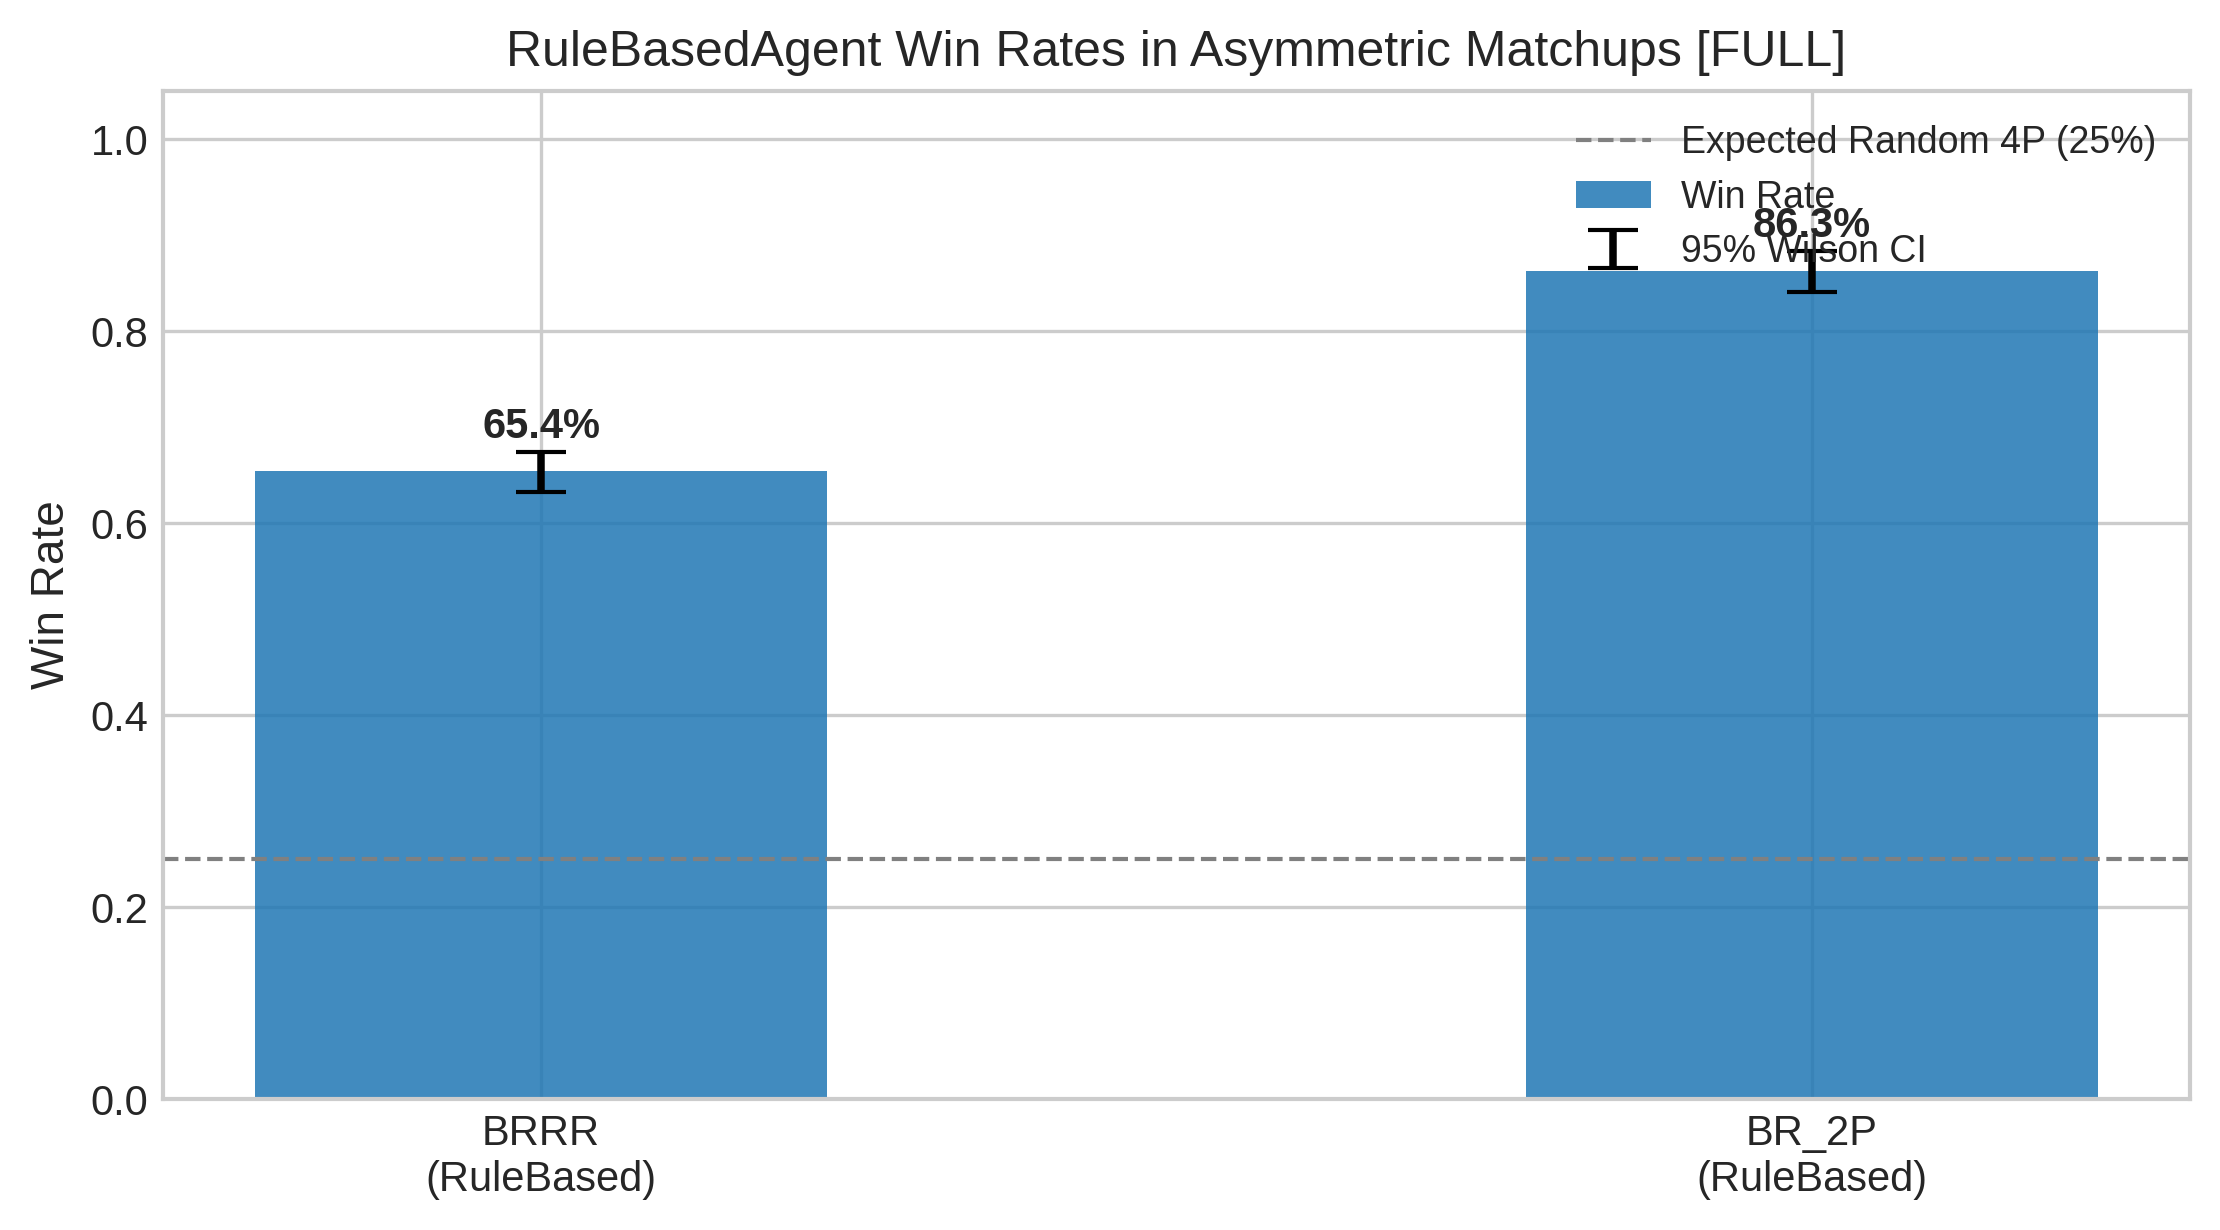
\includegraphics[width=0.85\linewidth]{figures/fig3_baseline_winrates_full.png}
\caption{Baseline Agent Win Rates with Wilson Score 95\% Confidence Intervals (EXP-03). RuleBased win rates in asymmetric 4-player BRRR (65.4\% [63.3\%, 67.5\%]) and 2-player BR\_2P (86.3\% [84.0\%, 88.3\%]), relative to the 25\% fair-share reference line.}
\label{fig:fig3_baseline_winrates}
\end{figure}




\subsection{Key Insights and Seating Fairness}
\begin{enumerate}
  \item \textbf{Asymmetric Heuristic Dominance:} In 4-player asymmetric competition (\texttt{BRRR}), the single \texttt{RuleBasedAgent} wins \textbf{$65.4\%$ of games} ($>2.6\times$ fair-share 25\%) with an average finishing rank of $1.61$. In heads-up play (\texttt{BR\_2P}), heuristic dominance reaches \textbf{$86.3\%$}.
  \item \textbf{Superseding the Pilot's 100\% Heads-Up Artifact:} In pilot testing ($n=20$), RuleBased won $20/20$ ($100.0\%$). Full-scale production ($n=1,000$) reveals that \texttt{RandomLegalAgent} wins \textbf{$13.7\%$ of heads-up games} (Wilson 95\% CI $[11.7\%, 16.0\%]$). This occurs when random play is dealt high-tempo opening hands (e.g., chains of compatible low cards) that exhaust before the heuristic agent can establish control.
  \item \textbf{Rigorous Seating Balance:} Seating equity was audited across all tournament games:
\end{enumerate}
\begin{itemize}
  \item In \texttt{BRRR}, RuleBased win rates across Seats 0, 1, 2, and 3 were $65.6\%$, $65.4\%$, $66.2\%$, and $64.4\%$ respectively ($\chi^2 = 0.58, p = 0.90$, no seat advantage).
  \item In \texttt{BR\_2P}, Player 0 won $50.7\%$ and Player 1 won $49.3\%$ ($\chi^2 = 0.20, p = 0.66$, no first-mover advantage).
\end{itemize}


\section{Experiment 4: Player-Count Scaling Dynamics}

\subsection{Objective and Setup}
EXP-04 examines how scaling participant count $N \in \{2, 3, 4, 5, 6\}$ affects environment dynamics. We executed $2,500$ games ($500$ games per player count) using \texttt{RandomLegalAgent} under matched random seeds (40000--40499) to eliminate deal variance.

\subsection{The Card Depletion Ratio \texorpdfstring{$\rho_0$}{rho\_0}}
In a standard 54-card deck with 6-card hands and 1 starting discard, the initial market size is:

\[
|M_0| = 54 - 1 - (N \times 6) = 53 - 6N
\]

The cards distributed among opponents are:

\[
|C_{\text{opp}}| = (N - 1) \times 6 = 6N - 6
\]

We formally define the initial card ratio $\rho_0$ (card depletion ratio $\rho_0$):

\[
\rho_0 = \frac{|C_{\text{opp}}|}{|M_0|} = \frac{6N - 6}{53 - 6N}
\]




\begin{table}[htbp]
\centering
\caption{Player Count Scaling Dynamics $N \in \{2..6\}$ (EXP-04, $N = 2{,}500$ episodes)}
\label{tab:exp04_scaling}
\small
\resizebox{\textwidth}{!}{%
\begin{tabular}{ccccccccc}
\toprule
$N$ & \textbf{Initial Market} $|M_0|$ & \textbf{Opponent Cards} $|C_{\text{opp}}|$ & \textbf{Ratio} $\rho_0$ & \textbf{Mean Turns} & \textbf{Turns/Player} & \textbf{Draws} & \textbf{Reshuffles} & \textbf{Trunc \%} \\
\midrule
2 & 41 & 6 & 0.146 & 63.9 & 31.9 & 35.2 & 0.41 & 0.0\% \\
3 & 35 & 12 & 0.343 & 102.3 & 34.1 & 65.2 & 1.97 & 0.4\% \\
4 & 29 & 18 & 0.621 & 489.6 & 122.4 & 438.0 & 244.37 & 41.4\% \\
5 & 23 & 24 & 1.044 & 702.9 & 140.6 & 572.5 & 163.04 & 54.6\% \\
6 & 17 & 30 & 1.765 & 793.3 & 132.2 & 760.4 & 631.53 & 74.6\% \\
\bottomrule
\end{tabular}%
}
\end{table}







\begin{figure}[htbp]
\centering
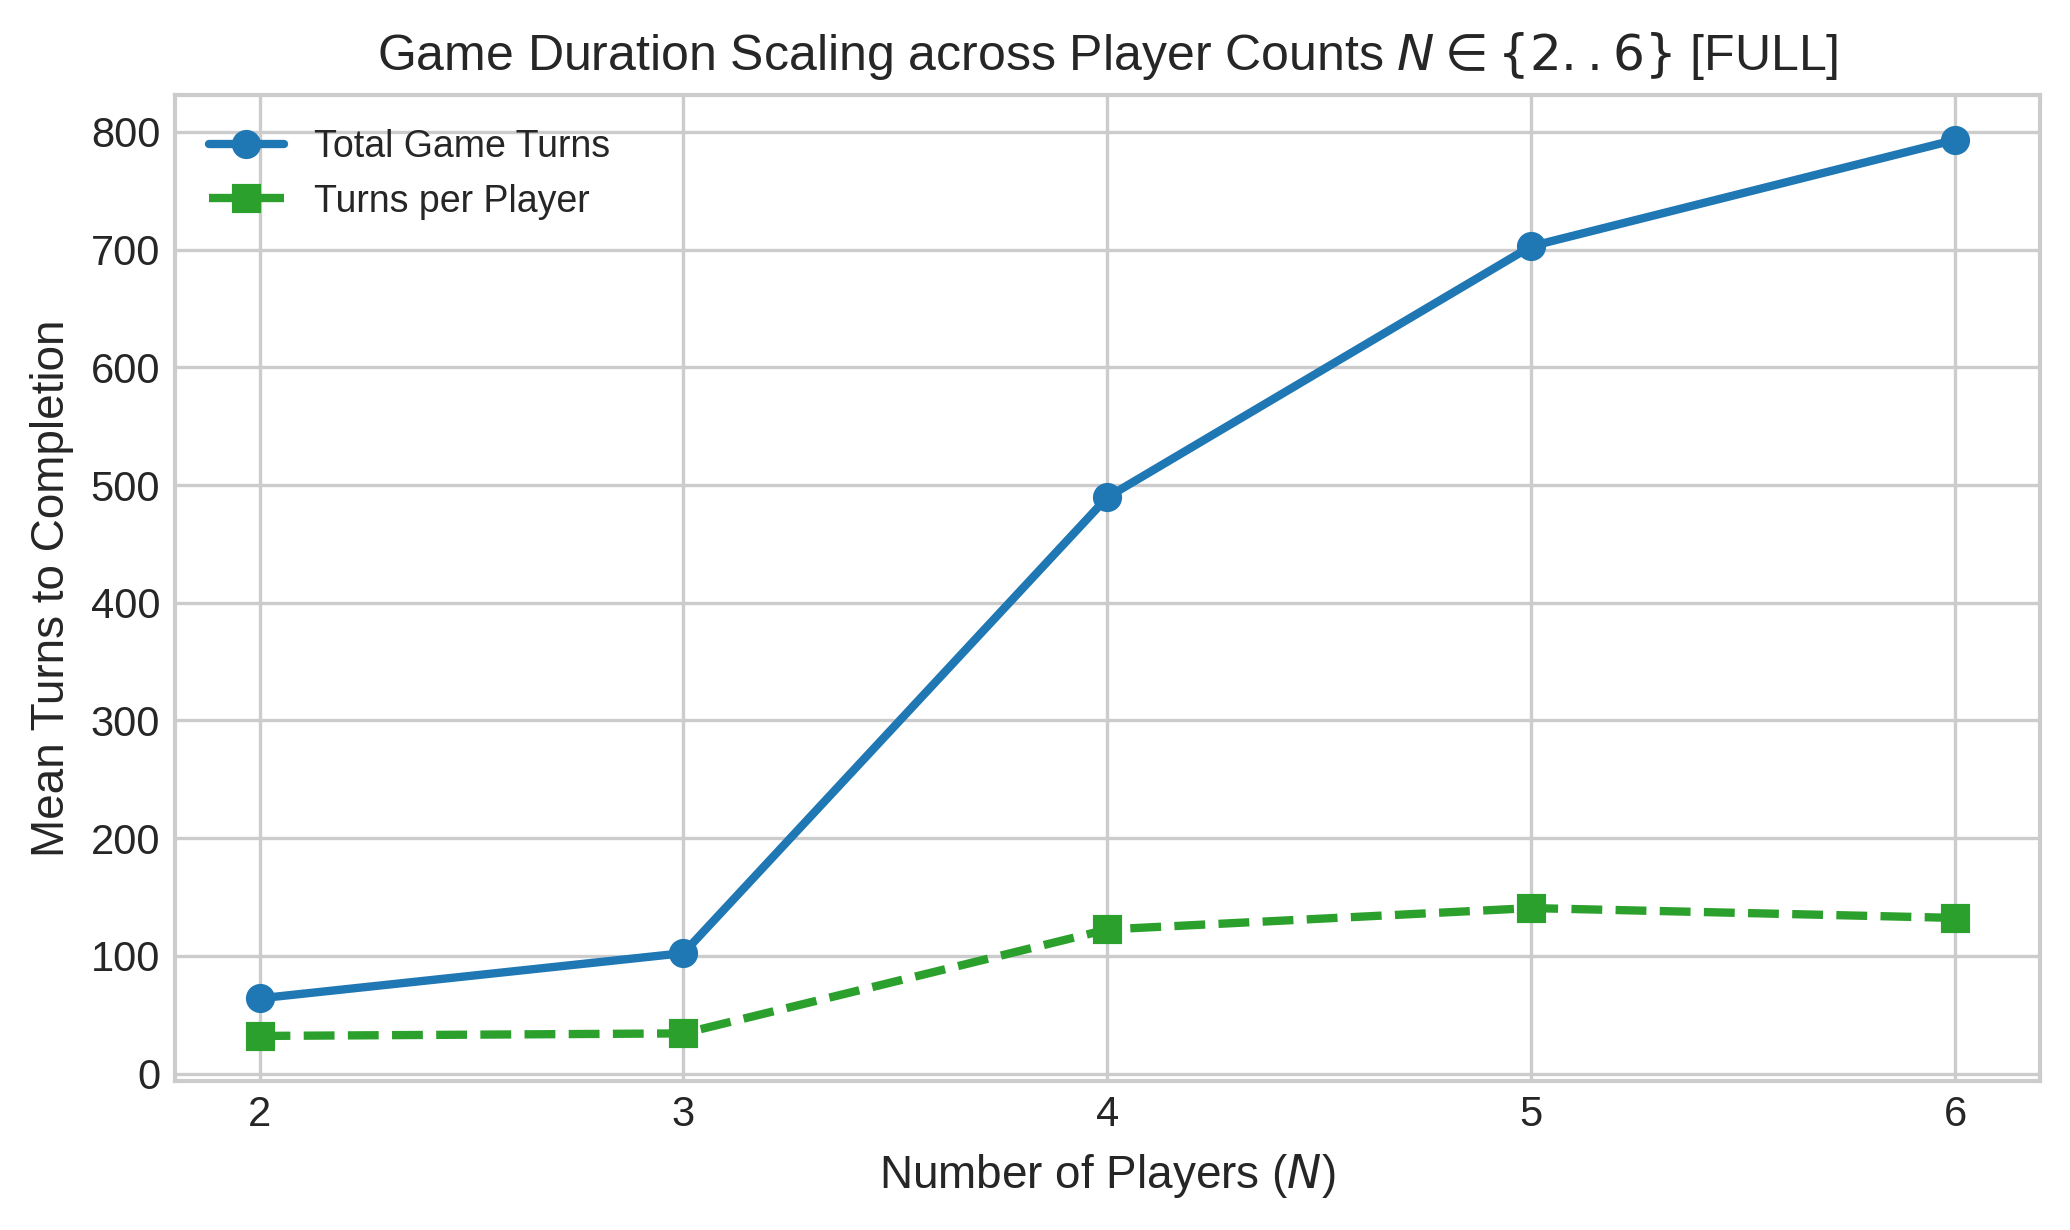
\includegraphics[width=\linewidth]{figures/fig4_player_scaling_full.png}
\caption{Player Count Scaling Dynamics across $N \in \{2..6\}$ (EXP-04). Total game duration and turns per player scaling across participant counts, highlighting the marked escalation and market exhaustion between $N=3$ and $N=4$ where $\rho_0$ approaches and exceeds unity.}
\label{fig:fig4_player_scaling}
\end{figure}




\subsection{Discussion: The Empirical Scaling Regime Shift}
The data demonstrates an empirical regime shift in gameplay dynamics:
\begin{itemize}
  \item \textbf{Abundant Market Regime ($N \le 3, \rho_0 < 0.5$):} The draw deck contains ample reserves ($|M_0| \ge 35$). Games resolve rapidly ($63.9$ to $102.3$ turns), market reshuffling is rare ($\le 1.97$ reshuffles), and truncations are virtually absent ($\le 0.4\%$).
  \item \textbf{Depleted Market Regime ($N \ge 5, \rho_0 > 1.0$):} At $N=5$ and $N=6$, opponent hands collectively exceed the opening market size ($\rho_0 = 1.044$ and $1.765$). The initial market is exhausted within the opening round of play, triggering massive discard recycling ($631.53$ reshuffles at $N=6$) and elevating the truncation rate to \textbf{$74.6\%$}.
\end{itemize}

\begin{quote}
\small \textbf{Framing Boundary:} We describe this behavior as an \textit{empirical regime shift in observed gameplay and computational dynamics}, avoiding unwarranted claims of a thermodynamic singularity or mathematical phase transition.
\end{quote}


\section{Experiment 5: Controlled Rule-Variant Ablations}

\subsection{Objective and Ablation Design}
EXP-05 evaluates the modularity of WHOT-ML by measuring how isolated rule modifications alter gameplay distributions. Using a 4-player asymmetric BRRR setup, we executed $2,500$ games ($500$ games per variant across identical matched seeds 50000--50499):
\begin{enumerate}
  \item \textbf{\texttt{VAR-BASE}:} Reference baseline rules.
  \item \textbf{\texttt{VAR-NO-STACK-2}:} Pick-2 multi-card penalty stacking disabled.
  \item \textbf{\texttt{VAR-NO-STACK-3}:} Pick-3 multi-card penalty stacking disabled.
  \item \textbf{\texttt{VAR-NO-DECL}:} Last-card declaration requirement disabled.
  \item \textbf{\texttt{VAR-PENALTY-2}:} Last-card declaration violation penalty escalated from Draw 1 to Draw 2.
\end{enumerate}




\begin{table}[htbp]
\centering
\caption{Controlled Rule Variant Ablations (EXP-05, $N = 2{,}500$ episodes)}
\label{tab:exp05_rule_variants}
\small
\resizebox{\textwidth}{!}{%
\begin{tabular}{llcccc}
\toprule
\textbf{Variant ID} & \textbf{Description} & \textbf{Mean Turns} & $\Delta$ \textbf{Turns vs Base} & \textbf{Cliff's} $\delta$ & \textbf{RuleBased Win \%} \\
\midrule
VAR-BASE & Baseline WHOT-NG-v1 default rules & 223.3 & --- & --- & 66.2\% \\
VAR-NO-STACK-2 & Pick-2 penalty stacking disabled & 223.3 & +0.0 & 0.00 & 66.2\% \\
VAR-NO-STACK-3 & Pick-3 penalty stacking disabled & 223.3 & +0.0 & 0.00 & 66.2\% \\
VAR-NO-DECL & Last-card declaration rule disabled & 173.4 & -49.9 & -0.13 & 53.4\% \\
VAR-PENALTY-2 & Declaration penalty increased Draw 2 & 221.7 & -1.6 & 0.00 & 69.6\% \\
\bottomrule
\multicolumn{6}{l}{\footnotesize \textit{Mean Draws:} VAR-BASE (151.2), VAR-NO-STACK-2 (151.2), VAR-NO-STACK-3 (151.2), VAR-NO-DECL (118.8), VAR-PENALTY-2 (150.4)} \\
\end{tabular}%
}
\end{table}







\begin{figure}[htbp]
\centering
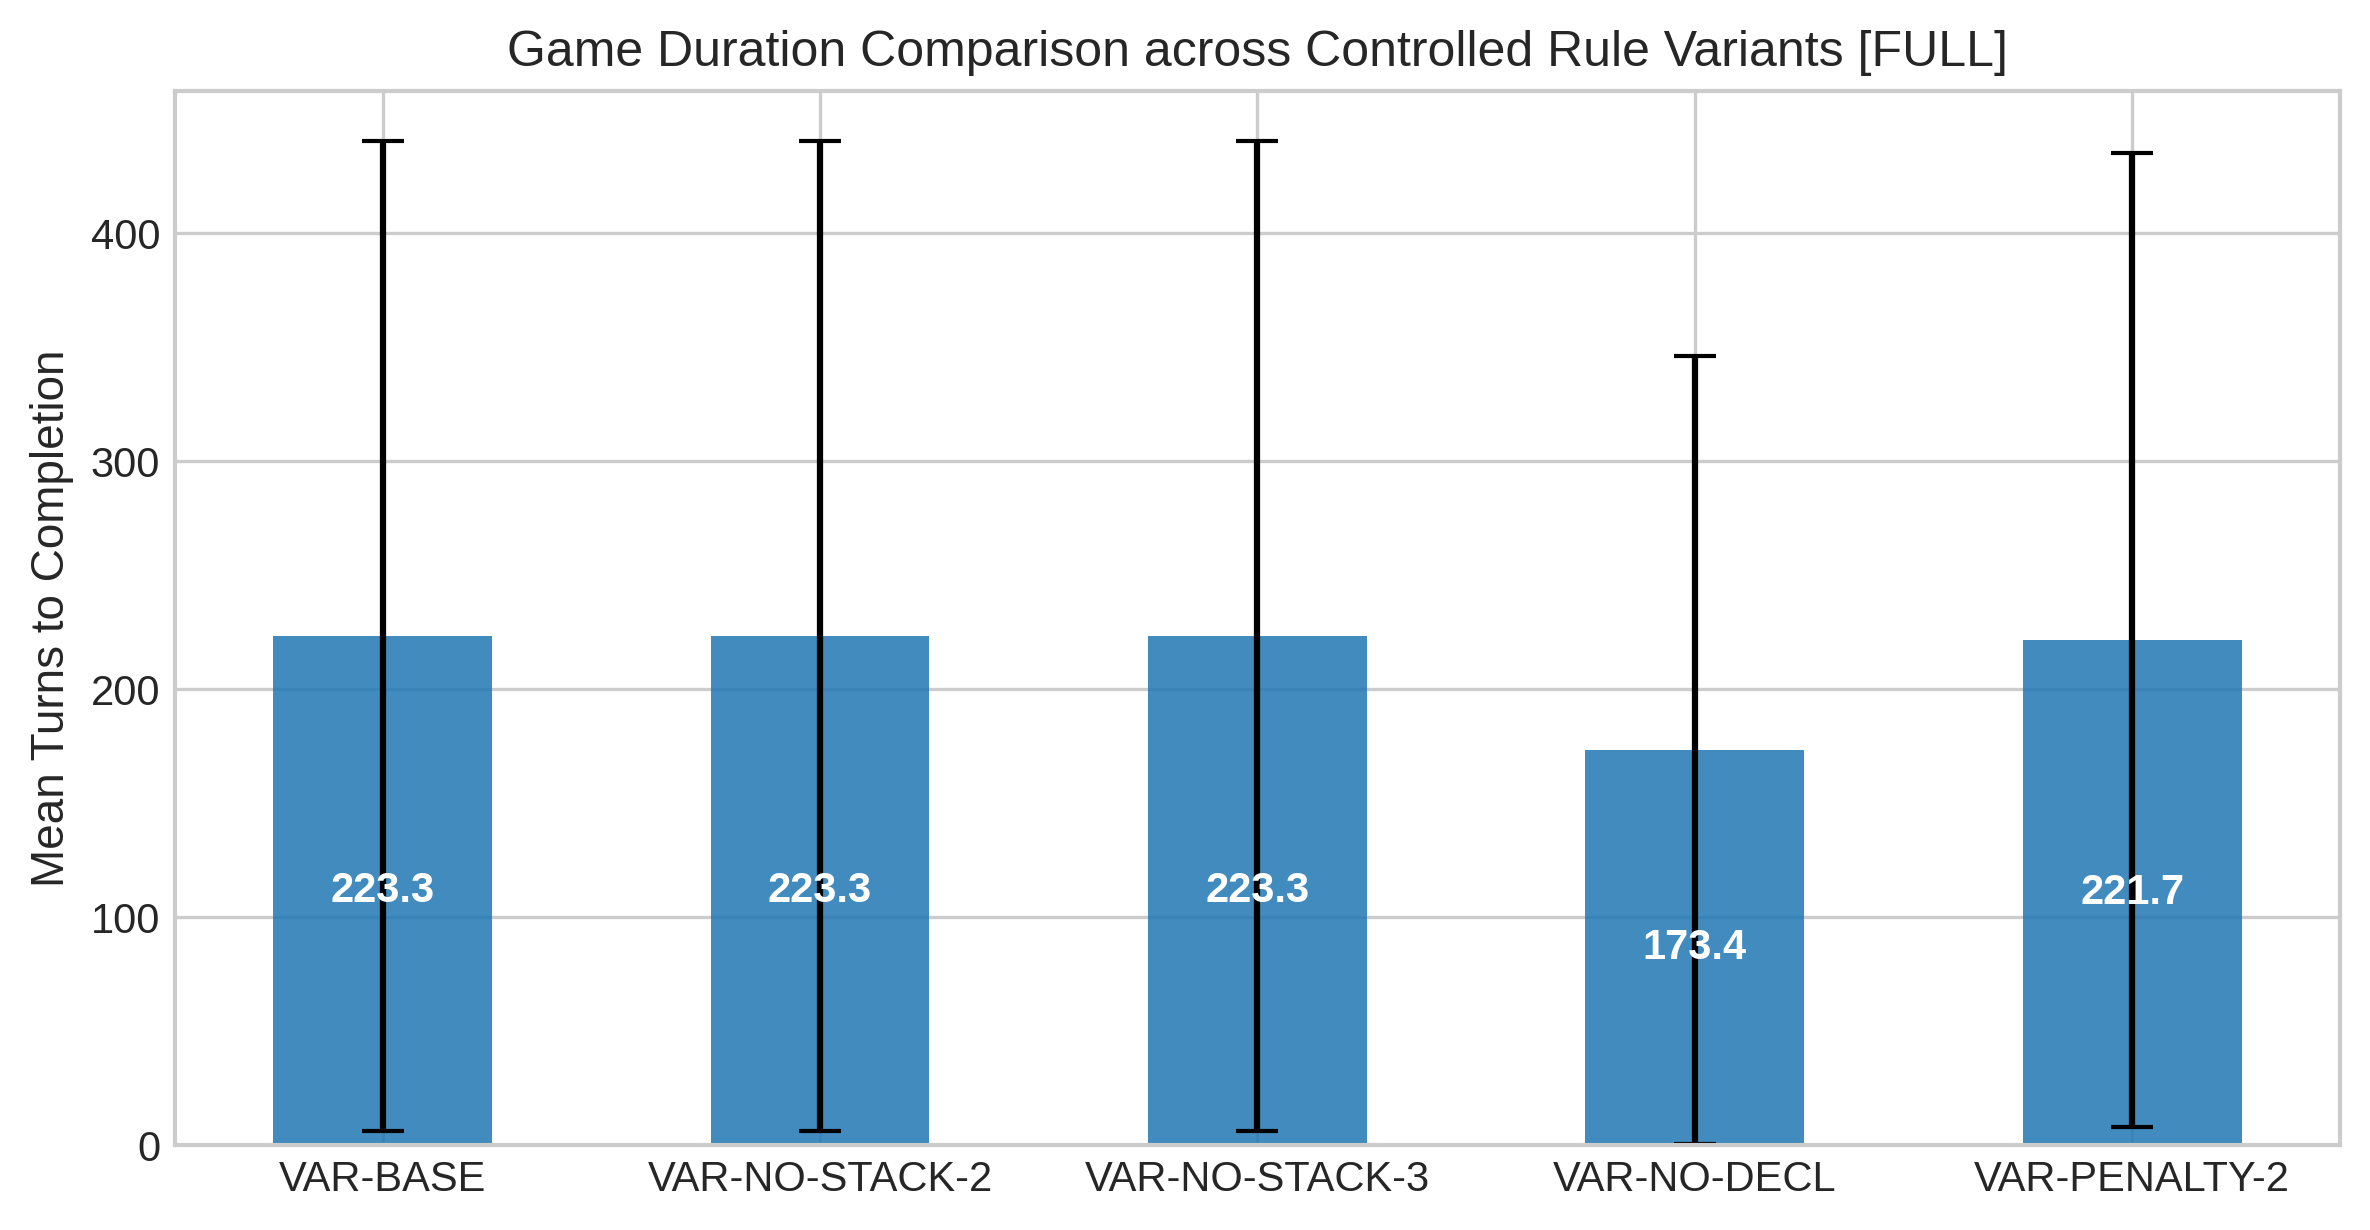
\includegraphics[width=0.85\linewidth]{figures/fig5_rule_variants_full.png}
\caption{Rule Variant Game Duration Distributions (EXP-05). Paired game duration distributions across five rule variants over 2,500 games (500 seeds each), showing the distinct shortening effect of removing the last-card declaration rule (\texttt{VAR-NO-DECL}).}
\label{fig:fig5_rule_variants}
\end{figure}




\subsection{Empirical Analysis of Rule Effects}
\begin{enumerate}
  \item \textbf{Last-Card Declarations Drive Strategic Friction:} Removing the declaration rule (\texttt{VAR-NO-DECL}) shortens average game duration by \textbf{$49.9$ turns} ($223.3 \to 173.4$ turns, Cliff's $\delta = -0.13$) and compresses RuleBased win rate from $66.2\%$ to $53.4\%$. In baseline WHOT, declarations impose penalty risk on opponents and provide vital public signaling that heuristic agents exploit.
  \item \textbf{Opponent-Policy Dependence of Stacking Invariance:} Disabling Pick-2 or Pick-3 stacking produced identical game durations ($\Delta = +0.0$ turns) and win rates ($66.2\%$) across all $500$ seeds.
\end{enumerate}
\textit{Causal Explanation:} Chaining penalty cards requires consecutive players to possess matching special cards and execute them sequentially. Uniform random agents distribute their plays arbitrarily across all legal options, making consecutive penalty stacking vanishingly rare.
\textit{Scientific Lesson:} Stacking invariance is an empirical finding of the \textit{tested opponent population}, proving that the behavioral expression of game rules is intrinsically coupled to agent competence.


\section{Experiment 6: Determinism \& Reproducibility Audit}

\subsection{Verification Protocol}
EXP-06 audits the bitwise determinism and checkpoint continuity of \texttt{WHOT-NG-v1.0} across $200$ rigorous evaluation tests:
\begin{itemize}
  \item \textbf{Sub-Protocol 6A (100 Independent Replays):} 100 complete games were executed from seeds 60000--60099. Trajectory tuples $(a_t, e_t, r_t, s_t, w)$ were serialized and SHA-256 hashed. Each episode was then independently re-executed from scratch with identical seeds.
  \item \textbf{Sub-Protocol 6B (100 Checkpoint Continuations):} 100 games were interrupted mid-game at turn $T=10$, serialized to JSON via \texttt{serialize\_state()}, restored into a clean environment via \texttt{restore\_state()}, and executed to completion. The post-restoration trajectory was compared against the uninterrupted baseline.
\end{itemize}




\begin{table}[htbp]
\centering
\caption{Determinism and State Checkpoint Restoration Audit (EXP-06, $N = 200$ tests)}
\label{tab:exp06_determinism}
\small
\begin{tabular}{llccc}
\toprule
\textbf{Sub-Protocol} & \textbf{Test Target} & \textbf{Tests Executed} & \textbf{Exact Matches} & \textbf{Success Rate} \\
\midrule
Sub-Protocol 6A & Independent Deterministic Replay & 100 & 100 & 100.0\% \\
Sub-Protocol 6B & Mid-Game Checkpoint Restoration & 100 & 100 & 100.0\% \\
\midrule
\textbf{Overall} & \textbf{Reproduction Success Rate (RSR)} & \textbf{200} & \textbf{200} & \textbf{100.0\%} \\
\bottomrule
\end{tabular}
\end{table}




\subsection{Result}
All 100 replays generated identical 64-character SHA-256 state digests. All 100 checkpoint restorations produced bitwise identical continuation paths, achieving a \textbf{Reproduction Success Rate ($\text{RSR}$) of $100.0\%$}. WHOT-NG-v1 satisfies zero-tolerance reproducibility for tree search and RL checkpointing.


\section{Synthesis of Empirical Results}

\textbf{Table 7} provides a consolidated synthesis of the full production campaign.




\begin{table*}[t]
\centering
\caption{Master Results Synthesis across EXP-01 through EXP-06 ($N = 12{,}350$ Total Runs)}
\label{tab:master_results_synthesis}
\small
\resizebox{\textwidth}{!}{%
\begin{tabular}{lclllc}
\toprule
\textbf{Exp} & \textbf{Workload} & \textbf{Primary Finding} & \textbf{Key Empirical Value} & \textbf{Statistical Support} & \textbf{Claim Status} \\
\midrule
EXP-01 & 2,000 & RuleBased expands legal branching factor; & Branching: 7.63 vs 2.42; & Mean $\pm$ SD, Median, & Established \\
       &       & self-play exhibits emergent defensive stall. & Truncation: 43.6\% vs 7.6\% & Wilson 95\% CIs & \\
\addlinespace
EXP-02 & 449   & Hidden state differences produce decisive & Divergence: 84.63\% (380/449); & Wilson 95\% CI & Established \\
       &       & rollout divergence under zero leakage. & Information leakage: 0.0\% & [81.0\%, 87.7\%], $p < 10^{-15}$ & \\
\addlinespace
EXP-03 & 5,000 & Heuristic agents dominate random play; & BRRR Win: 65.4\%; BR\_2P Win: 86.3\%; & Wilson 95\% CIs, & Established \\
       &       & random agents win 13.7\% in 2P. & Seat effects: $p = 0.90, p = 0.66$ & Chi-square fairness & \\
\addlinespace
EXP-04 & 2,500 & Gameplay dynamics undergo regime shift & Reshuffles: 0.41 $\to$ 631.53; & Paired matched seeds, & Established \\
       &       & when opponent cards exceed market ($\rho_0 > 1$). & Truncation: 0.0\% $\to$ 74.6\% & Monotonic scaling & \\
\addlinespace
EXP-05 & 2,500 & Declaration rule adds strategic friction; & NoDecl: $\Delta = -49.9$ turns; & Paired-sample seeds, & Established \\
       &       & stacking invariant under random opponents. & NoStack: $\Delta = +0.0$ turns & Cliff's delta = -0.13 & \\
\addlinespace
EXP-06 & 200   & Simulator provides flawless bitwise & Replays: 100/100; Checkpoints: & Bitwise SHA-256 state & Established \\
       &       & determinism and checkpoint continuity. & 100/100; RSR = 100.0\% & hash parity & \\
\bottomrule
\end{tabular}%
}
\end{table*}





\section{Discussion}

The empirical findings from WHOT-ML reveal five core insights for AI research in imperfect-information games:

\subsection{Partial Observability is Operationally Consequential}
In many synthetic benchmarks, partial observability is simulated by masking features of an underlying MDP. In WHOT-ML, hidden information is physical and intrinsic. EXP-02 proves that unobserved card distributions are not dormant: an $84.63\%$ trajectory divergence rate under identical observations establishes that latent state differences immediately impact future game flow. Effective play in WHOT requires maintaining probability distributions over unobserved cards.

\subsection{Opponent Policies Shape the Effective Environment}
The experimental campaign demonstrates that environment dynamics cannot be decoupled from the agent population. In EXP-01 and EXP-03, greedy defensive heuristics produced an emergent 43.6\% truncation stall that never appeared under random play. In EXP-05, multi-card penalty stacking was behaviorally invisible ($\Delta = 0.0$) against random agents who failed to chain cards. The expression of the environment's complexity depends directly on the strategic competence of participating policies.

\subsection{Structural Scarcity Regimes in Multi-Agent Games}
EXP-04 demonstrates how game-theoretic dynamics shift as a function of physical resources. When the initial card ratio $\rho_0 = |C_{\text{opp}}| / |M_0|$ exceeds unity ($N \ge 5$), the draw market is exhausted before all players complete a single round, triggering massive discard recycling and prolonged games. This identifies player seating and deck sizing as critical hyper-parameters in card-game environments.

\subsection{Rules as Modular Experimental Controls}
By formalizing rules as modular configurations, WHOT-ML enables controlled scientific ablations. EXP-05 isolates the exact impact of cultural rule variations, proving that last-card declarations contribute roughly $50$ turns of gameplay and provide critical public signaling.

\subsection{Reproducibility as a Foundational Instrument Property}
Flawless bitwise determinism and state restoration ($100.0\%$ RSR across 200 trials) ensure that WHOT-ML can serve as a dependable testbed for algorithms requiring exact tree rollouts (MCTS), counterfactual evaluations (CFR), and reinforcement learning checkpointing.


\section{Limitations}

To maintain scientific integrity, several explicit limitations must be acknowledged:
\begin{enumerate}
  \item \textbf{Baseline Agent Scope:} Evaluation was conducted using uniform random and greedy heuristic agents. WHOT-ML Paper 1 does not present trained deep reinforcement learning agents; learning curves and sample efficiency are reserved for future work.
  \item \textbf{Absence of an Optimal Oracle:} In EXP-02, trajectory divergence was evaluated under a heuristic policy over a finite 20-step horizon. We do not claim that optimal actions differ between observationally equivalent states.
  \item \textbf{Emergent Heuristic Truncation:} The 43.6\% truncation rate in 4-player heuristic self-play reflects the limitations of simple greedy heuristics that lack multi-step cooperative or card-dumping strategies.
  \item \textbf{Opponent-Dependent Ablations:} Rule variant ablations were evaluated within a BRRR tournament structure against random opponents; stacking effects may manifest differently under competent policies.
  \item \textbf{No Human Parity Claims:} No human trials were conducted; baseline win rates establish behavioral reference floors, not human-level performance.
\end{enumerate}


\section{Future Work and Research Roadmap}

WHOT-ML provides the experimental laboratory for a multi-stage research roadmap:
\begin{itemize}
  \item \textbf{Paper 2 --- Reinforcement Learning in WHOT:} Benchmarking model-free RL (PPO, DQN), self-play algorithms, and Counterfactual Regret Minimization (CFR) within WHOT-NG-v1.
  \item \textbf{Paper 3 --- Hidden-Hand Belief Estimation:} Investigating auxiliary neural prediction heads $P(c \in H_j \mid \mathcal{H}_t^{\text{public}})$ to estimate hidden opponent hands from public discard histories.
  \item \textbf{Paper 4 --- Adaptive Opponent Modeling:} Developing meta-learning and recurrent architectures that infer opponent styles (e.g. aggressive penalty hoarding vs. conservative suit matching) and adapt policies online.
  \item \textbf{Subsequent Directions:} Evaluating zero-shot generalization across modular rule variants and investigating human-agent interactive play.
\end{itemize}


\section{Conclusion}

We have presented \textbf{WHOT-ML}, a formal, deterministic, and configurable reinforcement learning environment based on the widely played card game in Nigeria. Formalized as a multi-agent POMDP, \texttt{WHOT-NG-v1.0} establishes an uncompromised information boundary that guarantees zero private-card leakage while capturing the rich strategic dynamics of imperfect information.

Across an extensive $12,350$-run production campaign, we demonstrated that:
\begin{enumerate}
  \item Latent world state differences produce an $84.63\%$ trajectory divergence rate under identical observations;
  \item Heuristic policies dominate random play in asymmetric matchups ($65.4\%$ win rate in 4P, $86.3\%$ in 2P);
  \item Homogeneous heuristic self-play exposes an emergent defensive stall (43.6\% truncation rate) driven by retaliatory penalty loops and market recycling;
  \item Gameplay dynamics undergo an empirical regime shift as the opponent-to-market card ratio $\rho_0$ exceeds unity;
  \item Last-card declarations provide vital strategic friction, extending game duration by $49.9$ turns;
  \item The simulator achieves $100.0\%$ bitwise determinism and state-checkpoint continuity.
\end{enumerate}

By providing an open-source, mathematically grounded, and rigorously audited environment, WHOT-ML establishes a dependable scientific foundation for the next generation of algorithms reasoning under uncertainty, hidden information, and strategic multi-agent interaction.



\bibliographystyle{plainnat}
\bibliography{references}

\end{document}